To ensure that our prototype fulfills every requirements we set up in Chapter 3, we set up some testing scenarios, which we used to test the functionalities of our prototype. This scenario is made out of a maze/location like this

[top-view of maze/room here]

%TODO: Create top-view of room and conclude of test

%TODO: Show test findings

Therefore we can conclude that the test requirements set previously are all passed.

\begin{table}[H]
	\begin{tabular}{|l|l|}
		\hline
		\textbf{Requirement} & \textbf{Test} \\ \hline
		The rover can be controlled using a remote device. & PASSED/FAILED \\ \hline
		The rover should navigate autonomously through a maze. & PASSED/FAILED \\ \hline
		The laser sensor should make a usable 2D map of its surroundings. & PASSED/FAILED \\ \hline
	\end{tabular}
\end{table}

\clearpage
\section{Close proximity}

The first was to figure out the location of the rovers blind spots. To figure out what measuring angle the our specific sensors are using, a piece of paper with a ruler on was placed beneath the rover at a guide. The ultrasonic sensor test script from the appendix was then run multiple times to figure out when the object placed on the ruler was detected.

\begin{figure}[H]
	\centering
	\begin{subfigure}[H]{0.3\textwidth}
		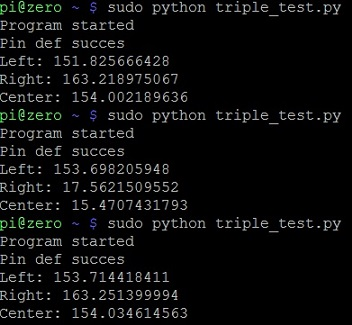
\includegraphics[width=\textwidth]{images/test-blindspotcmd.jpg}
		\subcaption{Blind spot readings}
	\end{subfigure}%
	\quad
	\begin{subfigure}[H]{0.3\textwidth}
		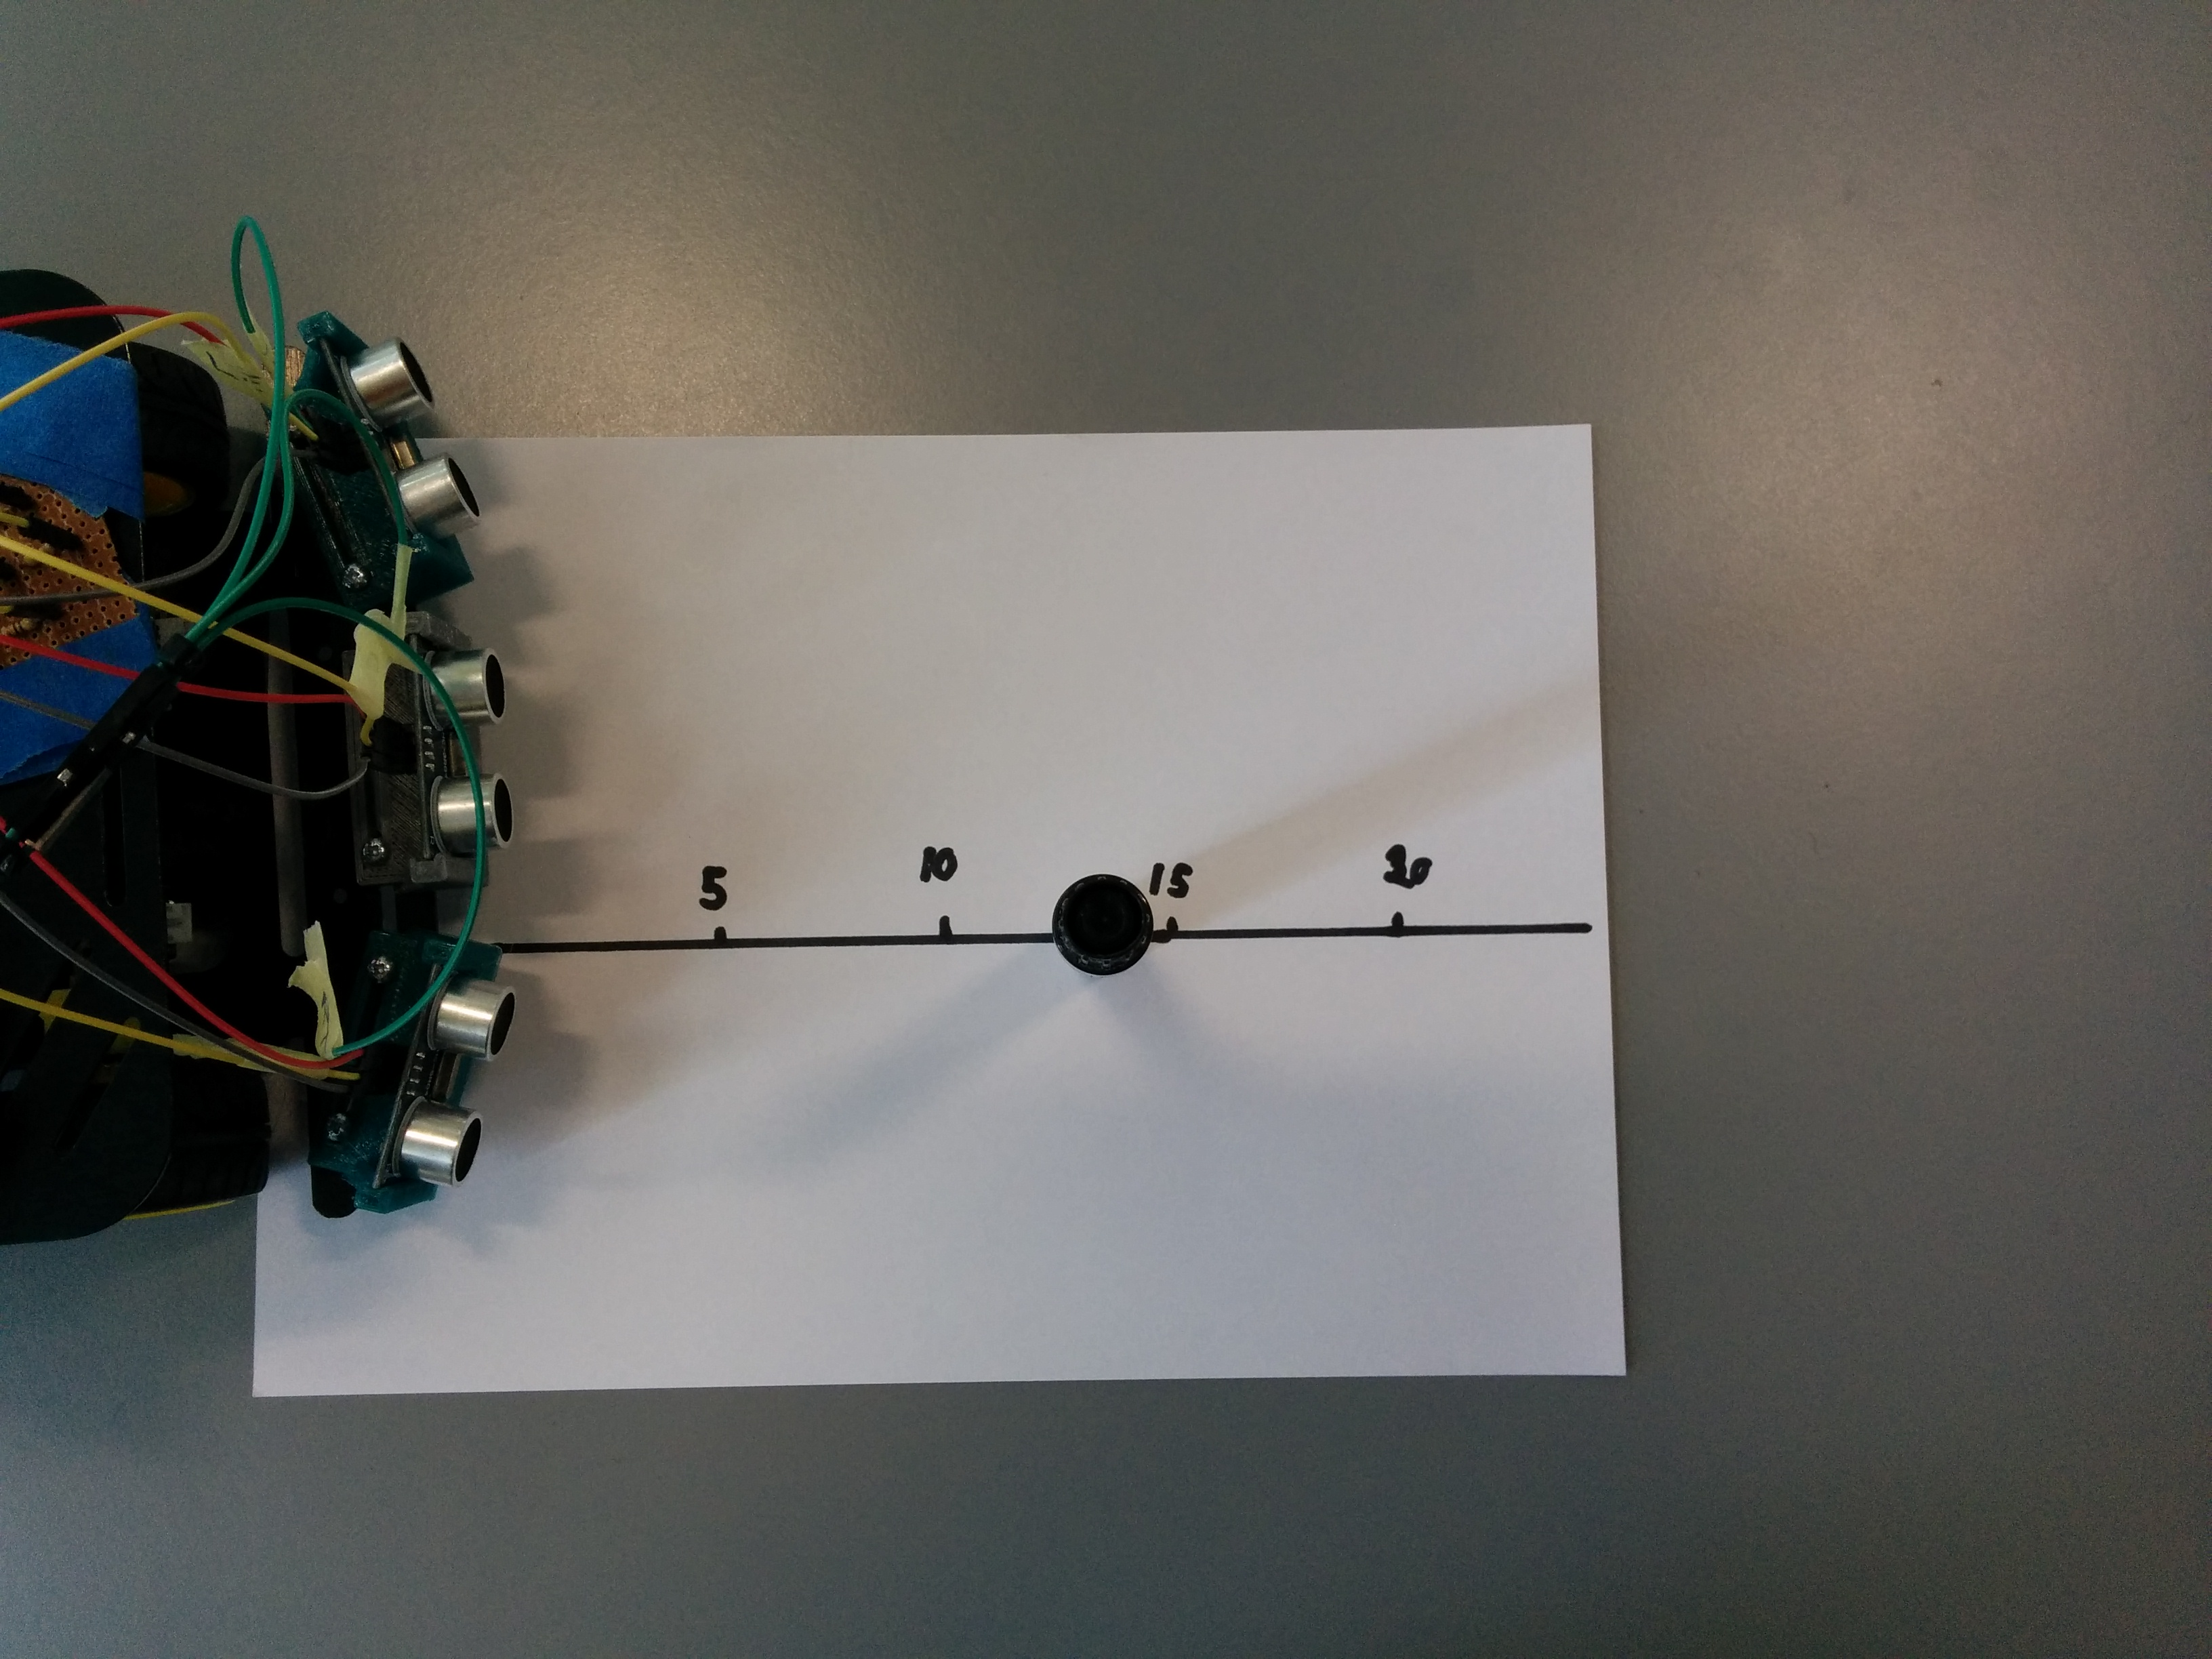
\includegraphics[width=\textwidth]{images/blindspot_test.jpg}
		\subcaption{Measuring the blind spot}
	\end{subfigure}%
	\quad
	\begin{subfigure}[H]{0.3\textwidth}
		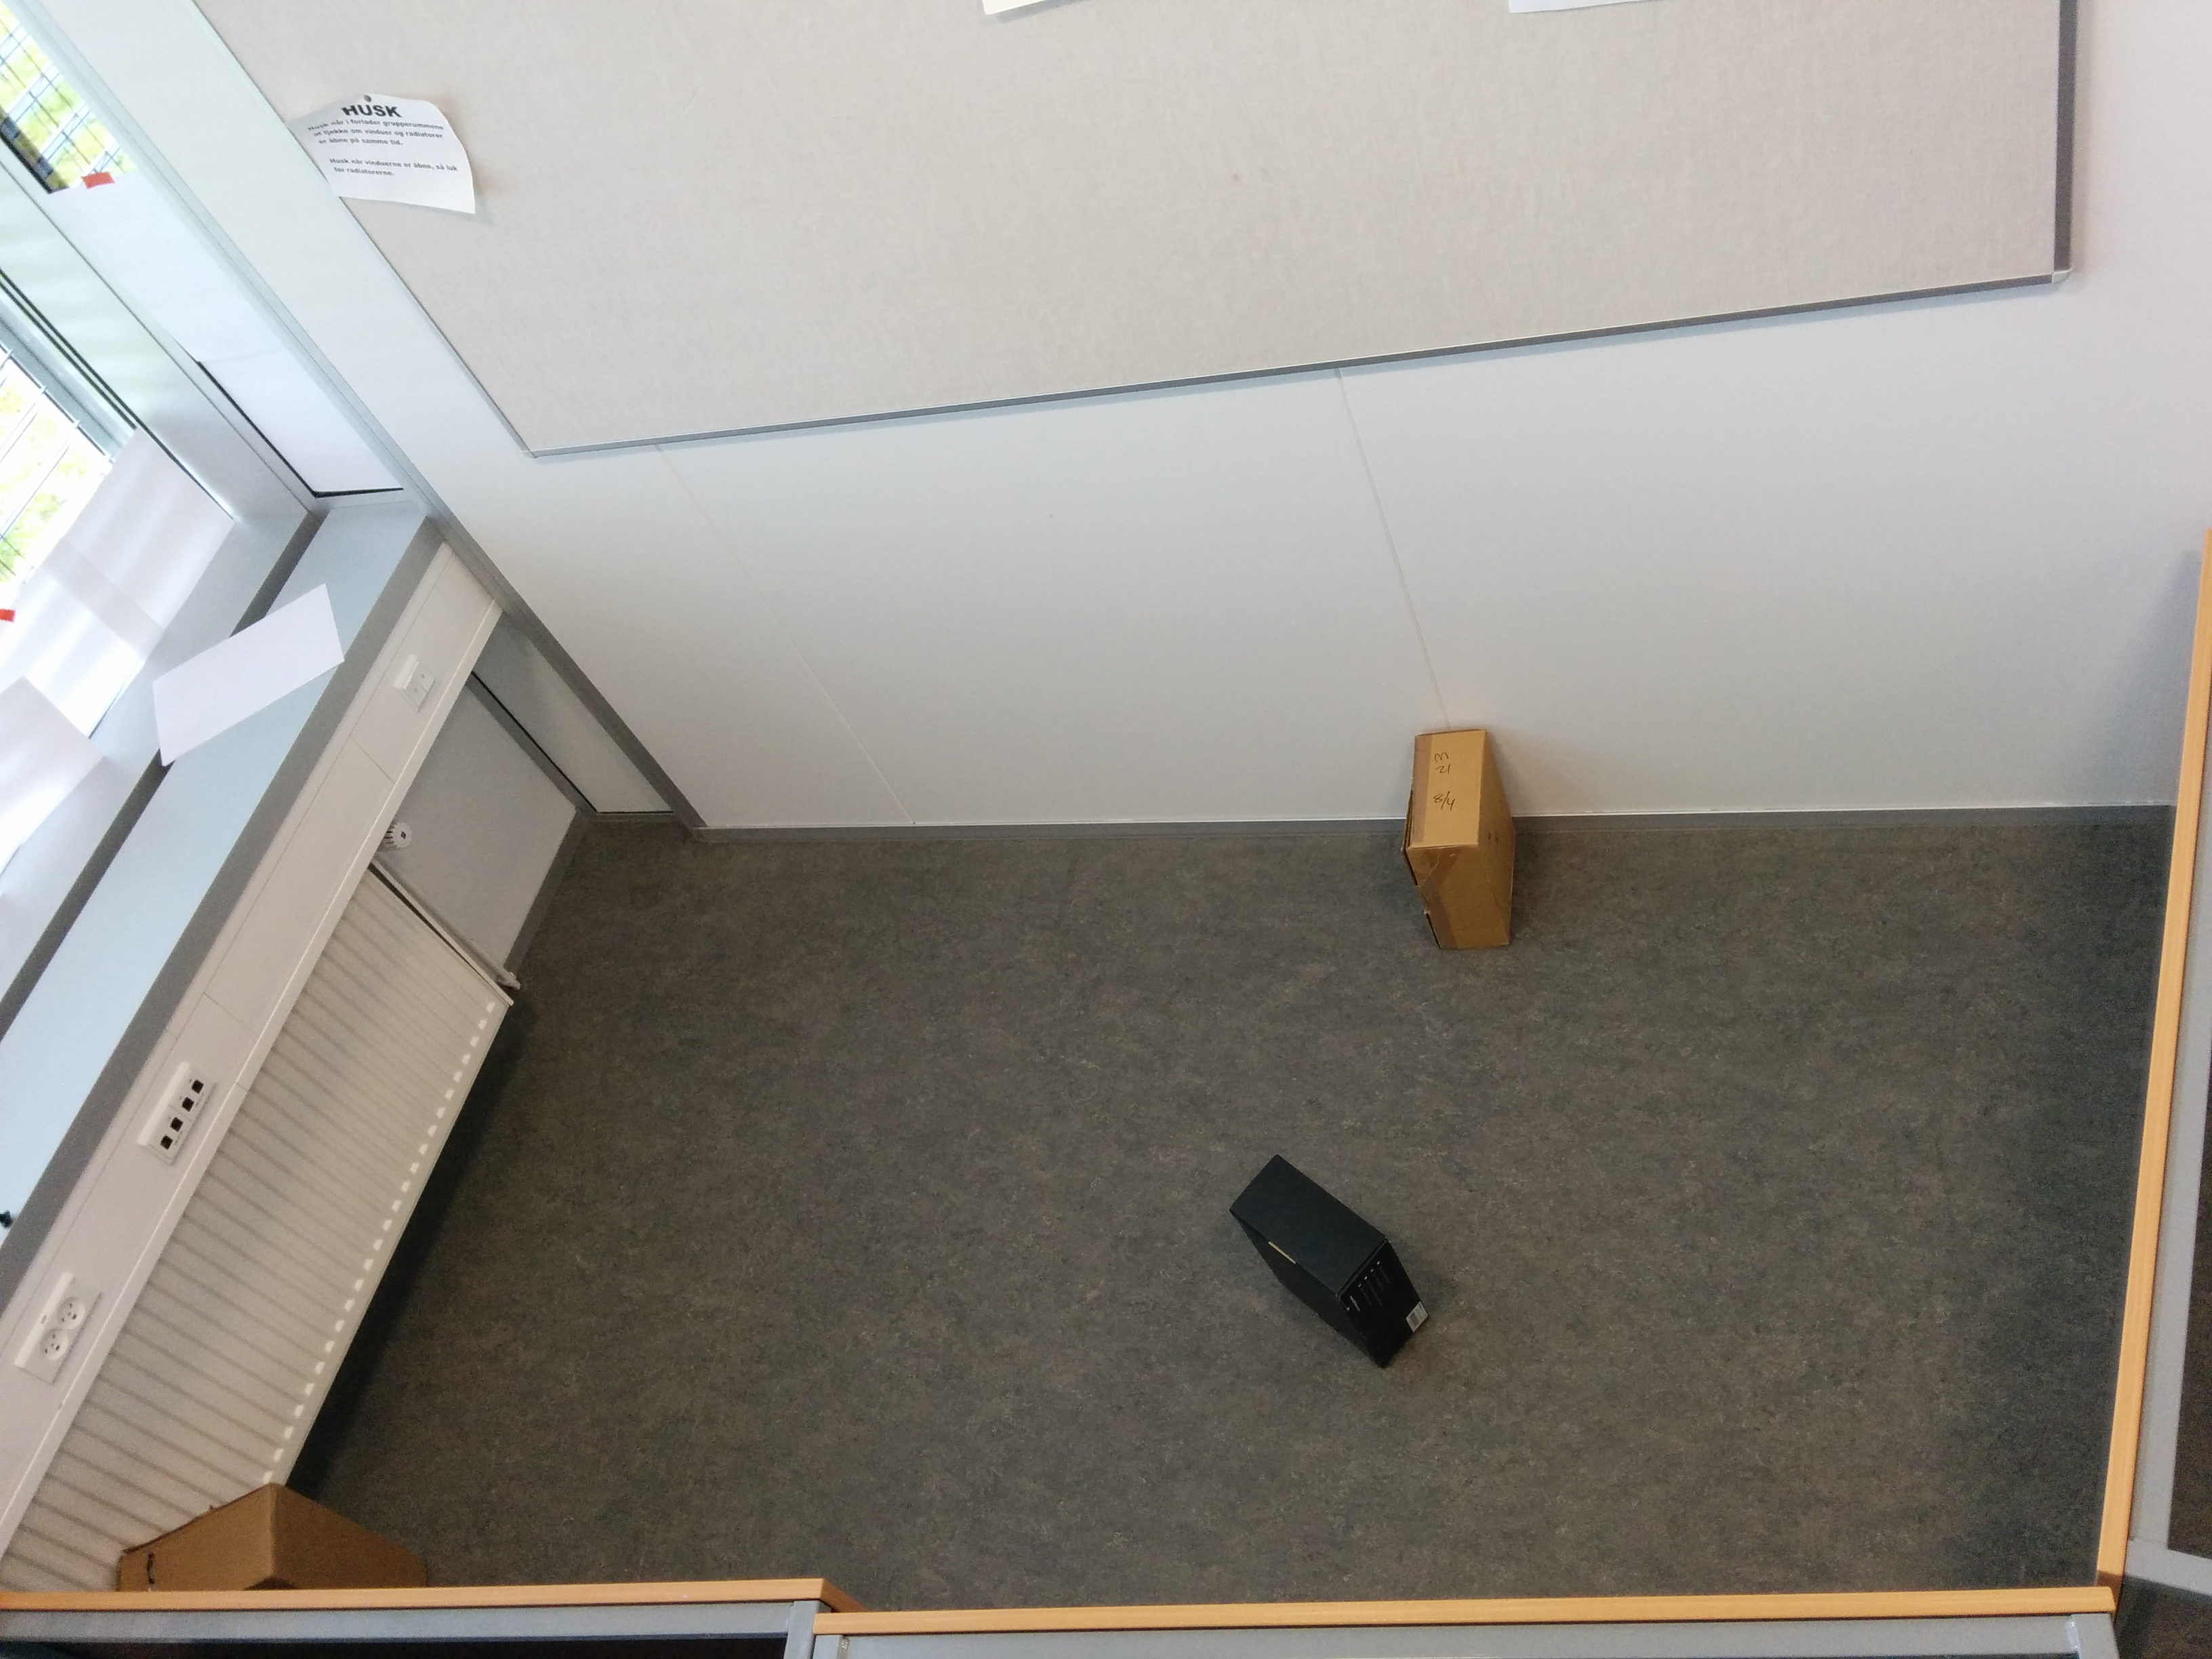
\includegraphics[width=\textwidth]{images/testing-course.jpg}
		\subcaption{The testing course}
	\end{subfigure}
\end{figure}

Through testing we determined that the ultrasonic sensors used for the particular project has a measuring angle of $15\degree$. This increases the rovers risk of running into a blind spot, since the blind areas are much larger than with the sensors with the larger viewing angle. The left-most figure shows the readings from the ultrasonic sensors, while the pen on the center figure was being moved back and forth. The center figure display where the tipping point(14.5cm from the sensors) is for the blind spot, if the test had been performed with a slimmer object compared to the pen, the blind spot threshold would be closer to the calculated one at around 19cm.\\
The testing course has been created arbitrarily, with the purpose of placing some objects for the rover to detect, avoid and navigate around.


When the distance threshold is set to a lower length (e.g 20cm), the rover ends up getting too close to objects before determining a new path. If the distance threshold is set to a high value (e.g 50cm), the rover has an easier time navigation/avoiding objects in its path, the downside is though that with a large distance threshold value, the rover never reaches certain parts of the course, because it detects today many nearby objects and therefore does not approach the area.

\clearpage
\begin{figure}[H]
	\centering
	\begin{subfigure}[H]{0.4\textwidth}
		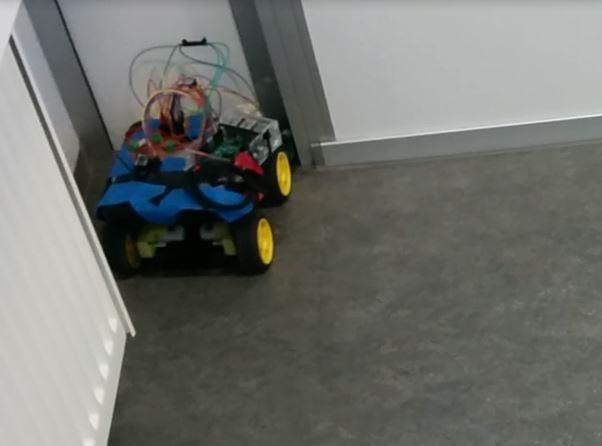
\includegraphics[width=\textwidth]{images/test-stuckincorner.jpg}
		\subcaption{}
	\end{subfigure}%
	\quad
	\begin{subfigure}[H]{0.4\textwidth}
		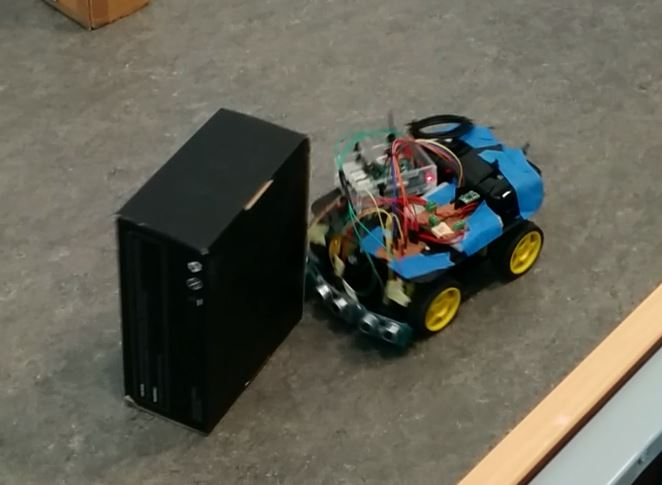
\includegraphics[width=\textwidth]{images/test-badmeasuringangle.jpg}
		\subcaption{}
	\end{subfigure}
\end{figure}

The current algorithm for the rover get stuck in a loop if the rover drives directly into a corner(figure a). The reason for the looping is that the distance towards to wall of either side of the rover are equal, so it can not determine which direction it should turn.\\
Because of the skewed angles of the object in the test course, the rover would sometimes hit them. Figure b clear shows the rover hitting the object face on, because the ultrasonic sensors were not able to read the distance to the walls of the box because they are at an angle.

When the rover turned to avoid the walls and other objects, it would skid across the floor. This resulted in the rover not turning on the spot, therefore reducing the accuracy of the steering.